\documentclass[tikz]{standalone}
\usepackage{amsmath}
\definecolor{bg}{HTML}{171D2B}
\definecolor{acc}{HTML}{F7B538}
\definecolor{line}{HTML}{8B93A7}
\begin{document}
\pagecolor{bg}
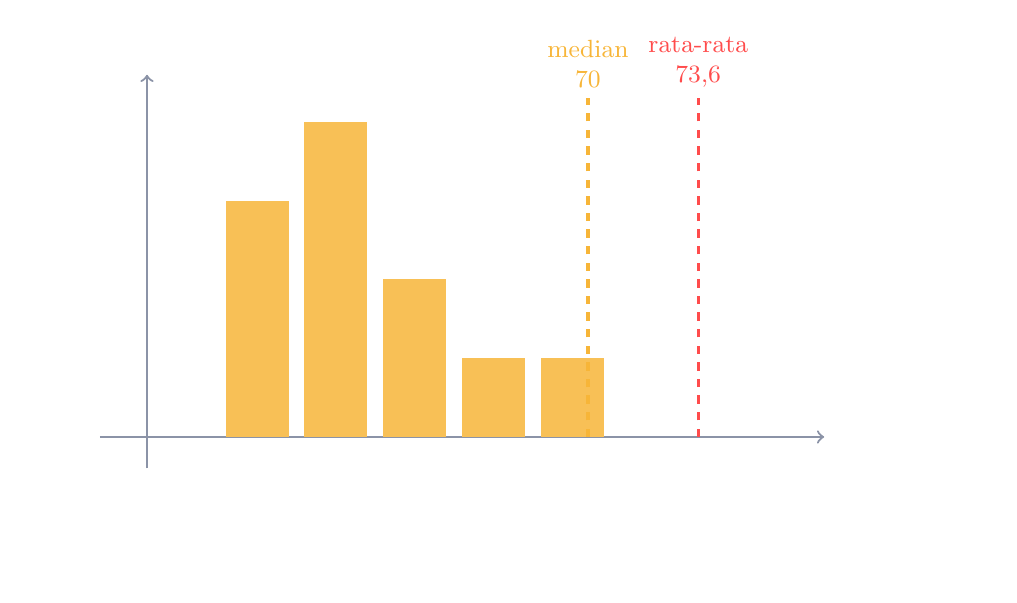
\begin{tikzpicture}[x=1cm,y=1cm]
  \draw[line,thick,->] (-0.6,0) -- (8.6,0) node[below right,white,font=\small] {nilai ulangan};
  \draw[line,thick,->] (0,-0.4) -- (0,4.6) node[left,white,font=\small] {frekuensi};
  \foreach \x/\h in {1/3,2/4,3/2,4/1,5/1}{
    \fill[acc!85] (\x,0) rectangle (\x+0.8,\h);
  }
  \foreach \x/\h/\t in {1/3/3,2/4/4,3/2/2,4/1/1,5/1/1}{
    \node[white,font=\small] at (\x+0.4,\h+0.25) {\t};
  }
  \foreach \x/\t in {1/60,2/70,3/80,4/90,5/100}{
    \node[white,font=\small] at (\x+0.4,-0.35) {\t};
  }
  \draw[red!70,very thick,dashed] (7.0,0) -- (7.0,4.3) node[above,red!70,font=\small,align=center] {rata-rata\\$73{,}6$};
  \draw[acc,very thick,dashed] (5.6,0) -- (5.6,4.3) node[above,acc,font=\small,align=center] {median\\$70$};
  \node[white,font=\small\itshape,align=left] at (5.6,-1.3) {nilai 100 dan 90 menarik rata-rata ke kanan,\\tetapi tidak menggeser median};
\end{tikzpicture}
\end{document}